\documentclass[11pt]{article}
\usepackage{geometry}
\usepackage[colorlinks]{hyperref}
\usepackage{graphicx}
\usepackage{mathpazo}
\usepackage[parfill]{parskip}

\makeatletter
\let \@sverbatim \@verbatim
\def \@verbatim {\@sverbatim \verbatimplus}
{\catcode`'=13 \gdef \verbatimplus{\catcode`'=13 \chardef '=13 }} 
\makeatother

\begin{document}

\textbf{CVEN 4333, Spring 2010, Assignment \#5, Due Friday February 12 at 5:00 in Cameron Bracken's mailbox. No late papers accepted.}

Please include the \textsf{R} script you create with this assignemnt.

\begin{enumerate}

%%%%%%%%%%%%%%%%%%%%%%%%%%%%%%%
%%%%%%%%%%%%%%%%%%%%%%%%%%%%%%%
\item Download the data files \texttt{colo\_monthly\_precip\_01.dat}, \texttt{colo\_monthly\_precip\_07.dat} from \url{http://cires.colorado.edu/~aslater/CVEN_6833/colo_pcp_monthly.html}. Also, download the file \texttt{colo\_dem.dat} from \url{http://cires.colorado.edu/~aslater/CVEN\_6833/colo_pcp.html} (same DEM data from the last assignment).  The first two files contains mean monthly total precipitation at 491 stations in colorado from 1980-2002 for the months of Januay and July.  The second file contains a DEM of colorado (same as last time). The web site describes the data format.  \textbf{Be aware that this data contains missing values that must be removed!}

One way to obtain estimates of rainfall on a regualar grid from irregualr points is to interpolate.   For observed data this is usually not a good way to go.  This is because (1) we are not using all we know about the data (namely that it varies spatially in a specific way) and (2) because it does not take into account the error associated with the data. 

While this is not a statistics class, statistical modeling is very common in hydrology.  A stistical approach can take into account the inherent error in the data.  Last time we visually saw that precipitation is correlated with spatiall and with elevation.  That is, there is some relationship

$$P = f(X,Y,Z) + \epsilon$$

where P is precipitation, $X$ is longitude, $Y$ is latitude, $Z$ is elevation and $\epsilon$ is the  error term.  Assumming that the function $f$ is linear, fit a model to the data in \textsf{R} using the \texttt{lm} function.  The model should have the form:

$$P = \beta_0 + \beta_1X+\beta_2Y+\beta_3Z + \epsilon.$$

Specifically, report the regression coefficients (the $\beta$'s), the standard error of each coefficient, the standard error of the fit ($\sigma_\epsilon$, standard deviation of the residuals) and the $R^2$ value. Is this fit statistically signifcant? Why? (Get this information from the \texttt{summary} function) Repeat this for both the January and July precipitation. 

\item Use the model from problem 1 to make a prediction of the rainfall at DEM grid points (use the \texttt{predict} function).  Plot a 3d surface of the predicted rainfall (using \texttt{plot.surface}) and an image plot with contours of precipitation. Repeat this for both the January and July precipitation. 

\item Plot the observed versus predicted precipitation for both January and July. Also plot the residuals versus X, Y, and Z (3 plots for each month, use the \texttt{residuals} function). Discuss the implications of these plots. 

\item Discuss the assumptions, advantages and disadvantages in using a linear model in part 1.  What other factors might contribut to precipitation that could improve this model. 

\item[{\it Extra Credit}] Use \texttt{interp} function from the \texttt{akima} package to linearly interpolate the precipitation to the DEM points.  Plot the interpolated surface, discuss the difference between this surface and the surface from the linear regression. Repeat this for both the January and July precipitation. 

\item Book problem 3.16
\item Book problem 3.18
\item Book problem 3.19
\item What is the probability that a 10 year flood will not be exceeded in any single year?
\item Snow in the most important form of precipitation on the Front range and predicting the characteristics of the spring melt is a formidable engineering problem. Through your own research indicate what each arrow in the diagram below (From left to right at the snow atmosphere interface and then left to right in the snow pack interior) would look like mathematically. Explain the mathematics in one English sentence for each arrow.

\end{enumerate}

\begin{figure}[htbp] %  figure placement: here, top, bottom, or page
   \centering
   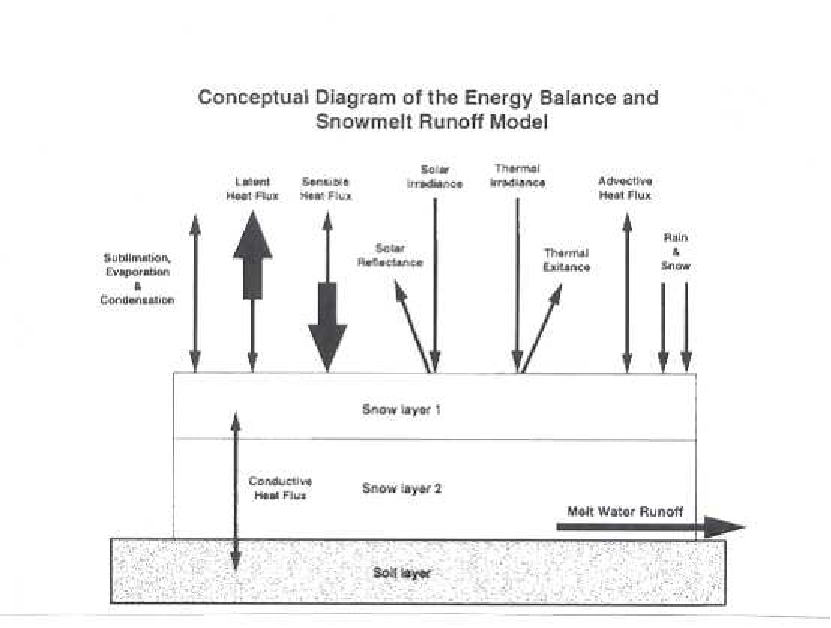
\includegraphics{snowmodel.pdf} 
   %\caption{example caption}
   %\label{fig:example}
\end{figure}

\end{document}  